\documentclass[11pt]{beamer}
\usetheme{CambridgeUS}
\usepackage[utf8]{inputenc}
\usepackage{amsmath}
\usepackage{amsfonts}
\usepackage{amssymb}
\usepackage{graphicx}
\usepackage{tikz}
\usepackage{color}
\usepackage{subfigure}
\usepackage[english]{babel}
\usepackage{tikz}
\usetikzlibrary{matrix}
%\usepackage[
%backend=biber,
%style=alphabetic,
%sorting=ynt
%]{biblatex}
\usepackage[numbers]{natbib}
%\addbibresource{{mps_group_a.bib}}
\setbeamertemplate{footline}
{
	\leavevmode
	\hbox{
		\begin{beamercolorbox}[wd=.5\paperwidth,ht=2.5ex,dp=1ex,left]{footline}
			\hspace*{2ex}AIMS Rwanda
		\end{beamercolorbox}
		\begin{beamercolorbox}[wd=.5\paperwidth,ht=2.5ex,dp=1ex,right]{footline}
			\insertframenumber{} / \inserttotalframenumber\hspace*{2ex}
		\end{beamercolorbox}
	}
	\vskip0pt
}
\title{Magic Squares}
\subtitle{Mathematical Problem Solving Presentation}

\author{
	Pearl KUURIDONG \\ Joelle SAFI \\ Abdelhakim MOUSTAPHA MAHAMAT \\ Latifah AKIMANA \\ Tchandikou OUADJA FARE}
\date{\today}	

\begin{document}
	
	%\begin{frame}
	\maketitle
	%\end{frame}
	
	\begin{frame}{OUTLINE}
		\begin{enumerate}
			\item PROBLEM STATEMENT
			\item DEFINITION OF MAGIC SQUARES
			\item TYPES OF MAGIC SQUARES
			\item SIAMESE ALGORITHM FOR ODD MAGIC SQUARE
			\item COMPLEMENTATION ALGORITHM FOR DOUBLY EVEN MAGIC SQUARE
			\item STRACHEY ALGORITHM FOR SINGLY EVEN MAGIC SQUARE
			%        \item REFERENCES
		\end{enumerate}
	\end{frame}
	
	\begin{frame}{Problem Statement}
		Imagine a $3 \times 3$ array of squares. The challenge is to put the integers 1 to 9, one in each square, so that each row and each column adds up to the same number. The best magic squares not only have all the rows and all the columns summing to the same number, but also the diagonals sum to the same number. How about $5 \times 5$ magic squares? Or even more \ldots
	\end{frame}
	
	\begin{frame}{Introduction}
		A \textbf{normal magic square} of order $n$ is an $n \times n$ grid filled with 
		the numbers $1,2,\dots,n^2$, such that:
		\begin{itemize}
			\item Each row has the same sum.
			\item Each column has the same sum.
			\item Both diagonals also have the same sum.
		\end{itemize}
		
		This common sum is called the \textbf{magic constant}.
	\end{frame}
	
	\begin{frame}{What is the Magic Constant?}
		The \textbf{magic constant $S$} is the number which each row, column, and diagonal must sum up to in the best magic squares.
		To compute it, we need the total sum of all numbers from $1$ to $n^2$.
	\end{frame}
	
	\begin{frame}{Classification of Magic Squares}
		There are 3 classifications of magic squares based on the methods to solve them:
		\begin{enumerate}
			\item Odd magic squares
			\item Doubly even magic squares
			\item Singly even magic squares
		\end{enumerate}
	\end{frame}
	
	\begin{frame}{The Siamese Algorithm (for odd $n$)}
		\textbf{Algorithm:}
		\begin{enumerate}
			\item Place $1$ in the middle of the top row.
			\item For each next number $k=2,3,\dots,n^2$:
			\begin{itemize}
				\item Move one step \textbf{up and to the right}.
				\item If this move goes outside the square, wrap around.
				\item If the target cell is filled, move \textbf{one step down}.
			\end{itemize}
		\end{enumerate}
	\end{frame}
	
	\begin{frame}{Siamese Algorithm for $3\times 3$ magic squares:}
		\begin{center}
			\begin{tikzpicture}[scale=2.0, every node/.style={font=\Large}]
				% Draw the grid once
				\draw (0,0) grid (3,3);
				
				% Row 1
				\node<2-> at (1.5,2.5) {1};
				\node<7-> at (2.5,2.5) {6};
				\node<9-> at (0.5,2.5) {8};
				
				% Row 2
				\node<4-> at (0.5,1.5) {3};
				\node<6-> at (1.5,1.5) {5};
				\node<8-> at (2.5,1.5) {7};
				
				% Row 3
				\node<10-> at (1.5,0.5) {9};
				\node<5-> at (0.5,0.5) {4};
				\node<3-> at (2.5,0.5) {2};
			\end{tikzpicture}
		\end{center}
	\end{frame}
	
	\begin{frame}{Complementation Algorithm (Doubly Even $n$)}
		\textbf{Applicable for:} $n$ multiple of 4, i.e., $n=4,8,12,\dots$
		
		\textbf{Algorithm:}
		\begin{enumerate}
			\item Fill the $n \times n$ square with numbers $1$ to $n^2$, row by row.
			\item Identify \textbf{special cells}:
			\begin{itemize}
				\item Cells on the main diagonals of each $4 \times 4$ sub-square.
				\item Corner cells of these sub-squares.
			\end{itemize}
			\item For \textbf{non-special cells}, replace each number $x$ by its complement:
			\[
			x \to n^2 + 1 - x
			\]
			\item The resulting square is a magic square.
		\end{enumerate}
	\end{frame}
	
	\begin{frame}{Complemenation Algorithm for $4 \times 4$ magic square}
		\transdissolve
		\only<1>{
			\begin{center}
				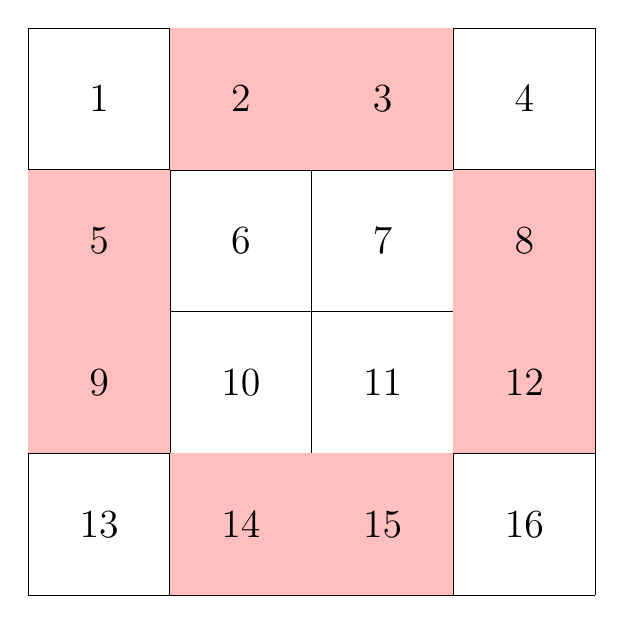
\begin{tikzpicture}[scale=1.8, every node/.style={font=\Large}]
					\draw (0,0) grid (4,4);
					% First version (maybe empty or partial filling)
					\fill[pink] (1,3) rectangle (3,4); 
					\fill[pink] (0,1) rectangle (1,3); 
					\fill[pink] (1,0) rectangle (3,1); 
					\fill[pink] (3,1) rectangle (4,3); 
					
					\node at (0.5,3.5) {1};
					\node at (1.5,3.5) {2};
					\node at (2.5,3.5) {3};
					\node at (3.5,3.5) {4};
					
					\node at (0.5,2.5) {5};
					\node at (1.5,2.5) {6};
					\node at (2.5,2.5) {7};
					\node at (3.5,2.5) {8};
					
					\node at (0.5,1.5) {9};
					\node at (1.5,1.5) {10};
					\node at (2.5,1.5) {11};
					\node at (3.5,1.5) {12};
					
					\node at (0.5,0.5) {13};
					\node at (1.5,0.5) {14};
					\node at (2.5,0.5) {15};
					\node at (3.5,0.5) {16};
				\end{tikzpicture}
			\end{center}
		}
		
		\only<2>{
			$$f(x) = n^2 + 1 - x$$
			\begin{center}
				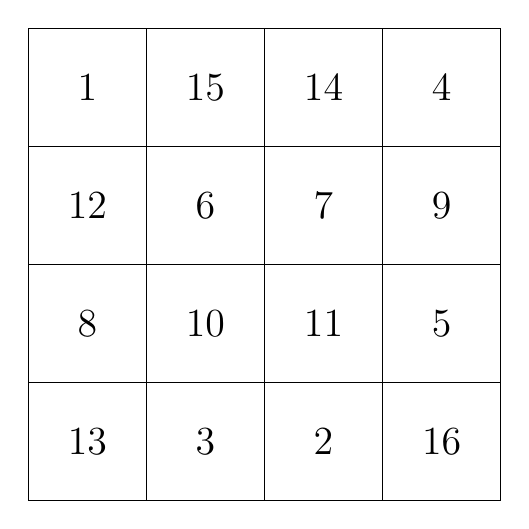
\begin{tikzpicture}[scale=1.5, every node/.style={font=\Large}]
					\draw (0,0) grid (4,4);
					\node at (0.5,3.5) {1};
					\node at (1.5,3.5) {15};
					\node at (2.5,3.5) {14};
					\node at (3.5,3.5) {4};
					
					\node at (0.5,2.5) {12};
					\node at (1.5,2.5) {6};
					\node at (2.5,2.5) {7};
					\node at (3.5,2.5) {9};
					
					\node at (0.5,1.5) {8};
					\node at (1.5,1.5) {10};
					\node at (2.5,1.5) {11};
					\node at (3.5,1.5) {5};
					
					\node at (0.5,0.5) {13};
					\node at (1.5,0.5) {3};
					\node at (2.5,0.5) {2};
					\node at (3.5,0.5) {16};
				\end{tikzpicture}
			\end{center}
		}
	\end{frame}
	
	\begin{frame}{Strachey's Algorithm (Singly Even $n$)}
		\textbf{Applicable for:} $n$ even but not multiple of 4, i.e., $n=6,10,14,\dots$
		
		\textbf{Algorithm:}
		\begin{enumerate}
			\item Divide the $n \times n$ square into four equal blocks of size $(n/2) \times (n/2)$.
			\item Construct a magic square of order $n/2$ (e.g., using the Siamese algorithm).
			\item Place this square in each block, adding an offset to each block:
			\begin{itemize}
				\item Top-left: $+0$
				\item Top-right: $+2 \cdot (n/2)^2$
				\item Bottom-left: $+3 \cdot (n/2)^2$
				\item Bottom-right: $+ (n/2)^2$
			\end{itemize}
			\item Swap certain columns and/or rows according to Strachey's rule:
			\begin{itemize}
				\item Select $k=n/4$ columns from left and right.
				\item Swap the elements of these columns between top and bottom blocks.
			\end{itemize}
			\item The resulting square is a magic square.
		\end{enumerate}
	\end{frame}
	
	
	\begin{frame}{Strachey Algorithm for $6 \times 6$ magic squares}
		\begin{center}
			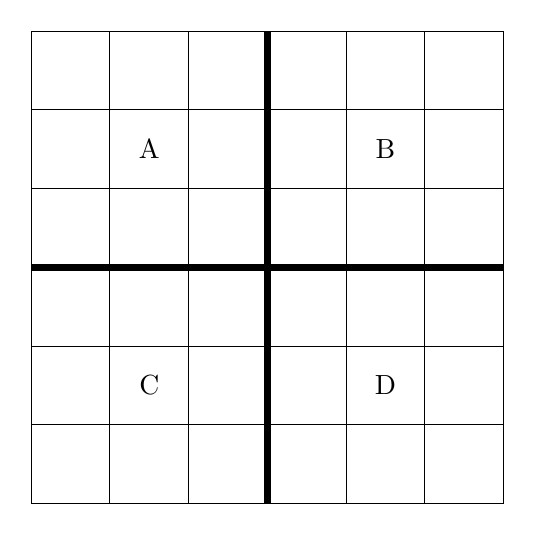
\begin{tikzpicture}[scale=1.0]
				\draw (0,0) grid (6,6);
				
				\draw[line width=2.5pt] (3,0) -- (3,6); 
				\draw[line width=2.5pt] (0,3) -- (6,3); 
				
				\node at (1.5,4.5) {A}; 
				\node at (4.5,4.5) {B}; 
				\node at (1.5,1.5) {C}; 
				\node at (4.5,1.5) {D}; 
			\end{tikzpicture}
		\end{center}
	\end{frame}
	
	\begin{frame}{Strachey Algorithm for $6 \times 6$ magic squares}
		\begin{center}
			\begin{tabular}{cc}
				\begin{minipage}{0.4\textwidth}
					\centering
					\textbf{A}\\[0.2cm]
					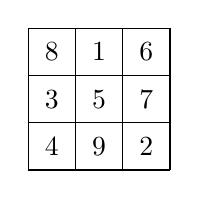
\begin{tikzpicture}[scale=0.6]
						\draw (0,0) grid (3,3);
						\node at (0.5,2.5) {8}; \node at (1.5,2.5) {1}; \node at (2.5,2.5) {6};
						\node at (0.5,1.5) {3}; \node at (1.5,1.5) {5}; \node at (2.5,1.5) {7};
						\node at (0.5,0.5) {4}; \node at (1.5,0.5) {9}; \node at (2.5,0.5) {2};
					\end{tikzpicture}
				\end{minipage}
				&
				\begin{minipage}{0.4\textwidth}
					\centering
					\textbf{B}\\[0.2cm]
					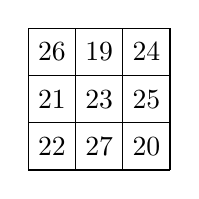
\begin{tikzpicture}[scale=0.6]
						\draw (0,0) grid (3,3);
						\node at (0.5,2.5) {26}; \node at (1.5,2.5) {19}; \node at (2.5,2.5) {24};
						\node at (0.5,1.5) {21}; \node at (1.5,1.5) {23}; \node at (2.5,1.5) {25};
						\node at (0.5,0.5) {22}; \node at (1.5,0.5) {27}; \node at (2.5,0.5) {20};
					\end{tikzpicture}
				\end{minipage}
				\\[2.0cm] 
				\begin{minipage}{0.4\textwidth}
					\centering
					\textbf{C}\\[0.2cm]
					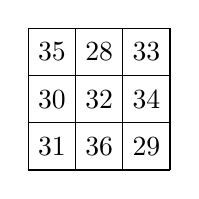
\begin{tikzpicture}[scale=0.6]
						\draw (0,0) grid (3,3);
						\node at (0.5,2.5) {35}; \node at (1.5,2.5) {28}; \node at (2.5,2.5) {33};
						\node at (0.5,1.5) {30}; \node at (1.5,1.5) {32}; \node at (2.5,1.5) {34};
						\node at (0.5,0.5) {31}; \node at (1.5,0.5) {36}; \node at (2.5,0.5) {29};
					\end{tikzpicture}
				\end{minipage}
				&
				\begin{minipage}{0.4\textwidth}
					\centering
					\textbf{D}\\[0.2cm]
					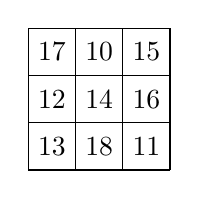
\begin{tikzpicture}[scale=0.6]
						\draw (0,0) grid (3,3);
						\node at (0.5,2.5) {17}; \node at (1.5,2.5) {10}; \node at (2.5,2.5) {15};
						\node at (0.5,1.5) {12}; \node at (1.5,1.5) {14}; \node at (2.5,1.5) {16};
						\node at (0.5,0.5) {13}; \node at (1.5,0.5) {18}; \node at (2.5,0.5) {11};
					\end{tikzpicture}
				\end{minipage}
			\end{tabular}
		\end{center}
	\end{frame}
	
	
	\begin{frame}{Strachey Algorithm for $6 \times 6$ magic squares}
		\begin{center}
			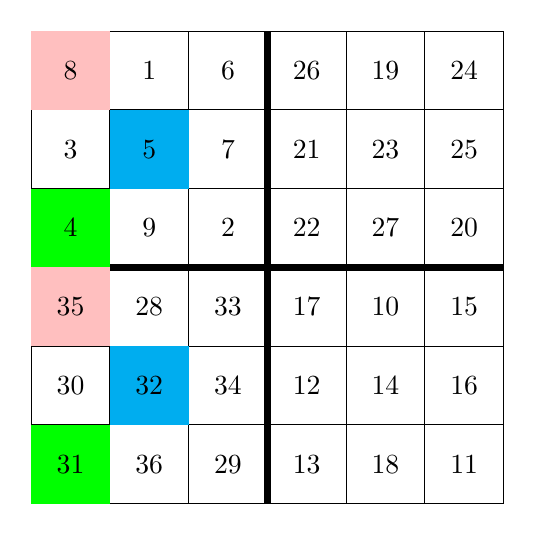
\begin{tikzpicture}[scale=1.0]
				\draw (0,0) grid (6,6);
				\draw[line width=2.5pt] (3,0) -- (3,6); 
				\draw[line width=2.5pt] (0,3) -- (6,3);
				
				\fill[pink] (0,2) rectangle (1,3); 
				\fill[pink] (0,5) rectangle (1,6); 
				%\fill[yellow] (0,3) rectangle (1,4); 
				\fill[yellow] (0,0) rectangle (1,1); 
				\fill[green] (0,3) rectangle (1,4); 
				\fill[green] (0,0) rectangle (1,1); 
				\fill[cyan] (1,4) rectangle (2,5); 
				\fill[cyan] (1,1) rectangle (2,2); 
				
				
				\node at (0.5,5.5) {8};
				\node at (1.5,5.5) {1};
				\node at (2.5,5.5) {6};
				\node at (3.5,5.5) {26};
				\node at (4.5,5.5) {19};
				\node at (5.5,5.5) {24};
				
				\node at (0.5,4.5) {3};
				\node at (1.5,4.5) {5};
				\node at (2.5,4.5) {7};
				\node at (3.5,4.5) {21};
				\node at (4.5,4.5) {23};
				\node at (5.5,4.5) {25};
				
				\node at (0.5,3.5) {4};
				\node at (1.5,3.5) {9};
				\node at (2.5,3.5) {2};
				\node at (3.5,3.5) {22};
				\node at (4.5,3.5) {27};
				\node at (5.5,3.5) {20};
				
				\node at (0.5,2.5) {35};
				\node at (1.5,2.5) {28};
				\node at (2.5,2.5) {33};
				\node at (3.5,2.5) {17};
				\node at (4.5,2.5) {10};
				\node at (5.5,2.5) {15};
				
				\node at (0.5,1.5) {30};
				\node at (1.5,1.5) {32};
				\node at (2.5,1.5) {34};
				\node at (3.5,1.5) {12};
				\node at (4.5,1.5) {14};
				\node at (5.5,1.5) {16};
				
				\node at (0.5,0.5) {31};
				\node at (1.5,0.5) {36};
				\node at (2.5,0.5) {29};
				\node at (3.5,0.5) {13};
				\node at (4.5,0.5) {18};
				\node at (5.5,0.5) {11};
			\end{tikzpicture}
		\end{center}
	\end{frame}
	
	\begin{frame}{$6\times 6$ magic square solved}
		\begin{center}
			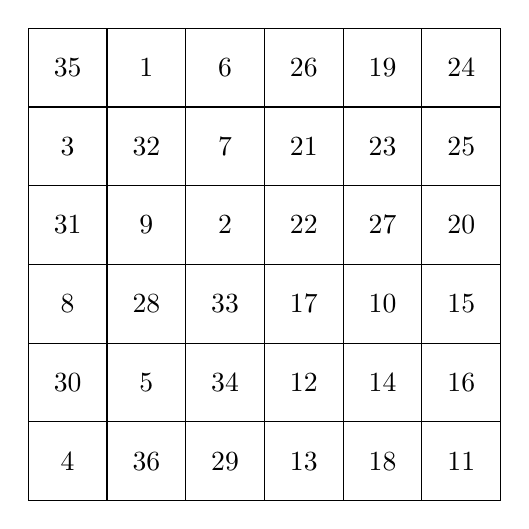
\begin{tikzpicture}[scale=1.0]
				\draw (0,0) grid (6,6);  
				%  \fill[pink] (1,3) rectangle (3,4); 
				% \fill[pink] (0,1) rectangle (1,3); 
				% \fill[pink] (1,0) rectangle (3,1); 
				% \fill[pink] (3,1) rectangle (4,3); 
				\node at (0.5,5.5) {35};
				\node at (1.5,5.5) {1};
				\node at (2.5,5.5) {6};
				\node at (3.5,5.5) {26};
				\node at (4.5,5.5) {19};
				\node at (5.5,5.5) {24};
				
				\node at (0.5,4.5) {3};
				\node at (1.5,4.5) {32};
				\node at (2.5,4.5) {7};
				\node at (3.5,4.5) {21};
				\node at (4.5,4.5) {23};
				\node at (5.5,4.5) {25};
				
				\node at (0.5,3.5) {31};
				\node at (1.5,3.5) {9};
				\node at (2.5,3.5) {2};
				\node at (3.5,3.5) {22};
				\node at (4.5,3.5) {27};
				\node at (5.5,3.5) {20};
				
				\node at (0.5,2.5) {8};
				\node at (1.5,2.5) {28};
				\node at (2.5,2.5) {33};
				\node at (3.5,2.5) {17};
				\node at (4.5,2.5) {10};
				\node at (5.5,2.5) {15};
				
				\node at (0.5,1.5) {30};
				\node at (1.5,1.5) {5};
				\node at (2.5,1.5) {34};
				\node at (3.5,1.5) {12};
				\node at (4.5,1.5) {14};
				\node at (5.5,1.5) {16};
				
				\node at (0.5,0.5) {4};
				\node at (1.5,0.5) {36};
				\node at (2.5,0.5) {29};
				\node at (3.5,0.5) {13};
				\node at (4.5,0.5) {18};
				\node at (5.5,0.5) {11};
			\end{tikzpicture}
		\end{center}
	\end{frame}
	
	\begin{frame}{Generalizations and Applications}
		Can we generalize this problem?
		\begin{itemize}
			\item Puzzle games (Sudoku)
		\end{itemize}
	\end{frame}
	
	\begin{frame}
		\begin{center}
			\Huge Thanks for listening!
		\end{center}
	\end{frame}
	
	
	\begin{frame}{References}
		\nocite{*}
		\bibliographystyle{apalike}
		\bibliography{mps_group_a} 
	\end{frame}
%	\begin{frame}[allowframebreaks]{References}
%		\nocite{*}
%		\printbibliography
%	\end{frame}
\end{document}
